\documentclass[12pt]{article}
\usepackage[margin=1in]{geometry}
\usepackage{amsmath,amssymb,amsthm}
\usepackage{graphicx}
\usepackage{hyperref}


\usepackage{subcaption}

\title{Phase 0}
\author{Tamzeed Elahi}
\date{\today}



\begin{document}
\maketitle

\section*{Project Description}
The problem I am interested for the class project is a system identification problem for a 2D quadrotor system. In the context of this course, the observability of this system will be evaluated; especially for estimating the input matrix which is unknown. 
\begin{align*}
    \dot{x} &= Ax + Bu + w \\
    y &= Cx + v
\end{align*} 
Here, the B matrix is unknown. \\\\
Ultimately, we would be able to estimate the B matrix using the observability matrix and consider the feasibility of a quadrotor system with additional controls (sliding/tilting) like \cite{Nemati2014}. 
\section*{Analytical model}
\begin{figure}[h!]
    \begin{subfigure}[t]{0.5\textwidth}
        \centering
        \includegraphics[width=5cm]{figures/model_diagram.png}
        \caption{Quadrotor system \cite{model_diagram}}
        \label{fig:01}
    \end{subfigure}
    \hfill
    \begin{subfigure}[t]{0.5\textwidth}
        \centering
        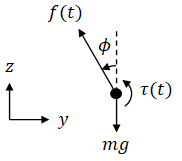
\includegraphics[width=5cm]{figures/free_body_diagram.png}
        \caption{Free body diagram \cite{model_diagram}}
        \label{fig:02}
    \end{subfigure}
\end{figure}
% \includegraphics[width=5cm]{model_diagram.png}

The state space model of a quadrotor system can be found in various literature\cite{K2019}\cite{Schreier2012}. For the class project, I will be using a simplified 2D model (only the y and z coordinates). The dynamic equation of the system can be estimated using Newton's second law of motion.
\begin{align*}
    \ddot{y} &= -\frac{1}{m}u_1(t) \sin{\phi} \\
    \ddot{z} &= -g + \frac{1}{m}u_1(t) \cos{\phi} \\ 
    \ddot{\phi} &= \frac{1}{I_{xx}}u_2(t) \\
\end{align*}
I assumed only two inputs (force and torque) are present in the system. Their relation with the states are nonlinear though it can be linearized with $\phi \approx 0$. It would be more interesting if the inputs are not forces and torques but rotor speeds. \\\\
States are: $x = [y, z, \dot{y}, \dot{z}, \phi, \dot{\phi}]^T$ \\\\
For now the output matrix-$C$ is considered to be an identity matrix. So, the system assumed to have a GPS and IMU sensors for full state estimation.

inputs are:
\begin{align*}
    u_1(t) &= F \\
    u_2(t) &= \tau
\end{align*}

\section*{matrix model:}
\begin{align*}
    \begin{bmatrix}
        \dot{y} \\
        \dot{z} \\
        \ddot{y} \\
        \ddot{z} \\
        \dot{\phi} \\
        \ddot{\phi} \\
        \dot{\beta_1} \\
        \dot{\beta_2} \\
        \dot{\beta_3} \\
    \end{bmatrix} &=
    \begin{bmatrix}
        0 & 0 & 1 & 0 & 0 & 0 & 0 & 0 & 0 \\
        0 & 0 & 0 & 1 & 0 & 0 & 0 & 0 & 0 \\
        0 & 0 & 0 & 0 & 0 & 0 & 0 & 0 & 0 \\
        0 & 0 & 0 & 0 & 0 & 0 & 0 & 0 & 0 \\
        0 & 0 & 0 & 0 & 0 & 1 & 0 & 0 & 0 \\
        0 & 0 & 0 & 0 & 0 & 0 & 0 & 0 & 0 \\
        0 & 0 & 0 & 0 & 0 & 0 & 0 & 0 & 0 \\
        0 & 0 & 0 & 0 & 0 & 0 & 0 & 0 & 0 \\
        0 & 0 & 0 & 0 & 0 & 0 & 0 & 0 & 0 \\
    \end{bmatrix}
    \begin{bmatrix}
        y \\
        z \\
        \dot{y} \\
        \dot{z} \\
        \phi \\
        \dot{\phi} \\
        \beta_1 \\
        \beta_2 \\
        \beta_3 \\
    \end{bmatrix} +
    \begin{bmatrix}
        0 & 0 \\
        \beta_1 & 0 \\
        0 & 0 \\
        \beta_2 & 0 \\
        0 & 0 \\
        0 & \beta_3 \\
        0 & 0 \\
        0 & 0 \\
        0 & 0 \\
    \end{bmatrix}
    \begin{bmatrix}
        F \\
        \tau \\
    \end{bmatrix} + w\\ \\
    &= 
    \begin{bmatrix}
        0 & 0 & 1 & 0 & 0 & 0 & 0 & 0 & 0 \\
        0 & 0 & 0 & 1 & 0 & 0 & 0 & 0 & 0 \\
        0 & 0 & 0 & 0 & 0 & 0 & 0 & 0 & 0 \\
        0 & 0 & 0 & 0 & 0 & 0 & 0 & 0 & 0 \\
        0 & 0 & 0 & 0 & 0 & 1 & 0 & 0 & 0 \\
        0 & 0 & 0 & 0 & 0 & 0 & 0 & 0 & 0 \\
        0 & 0 & 0 & 0 & 0 & 0 & 0 & 0 & 0 \\
        0 & 0 & 0 & 0 & 0 & 0 & 0 & 0 & 0 \\
        0 & 0 & 0 & 0 & 0 & 0 & 0 & 0 & 0 \\
    \end{bmatrix}
    \begin{bmatrix}
        y \\
        z \\
        \dot{y} \\
        \dot{z} \\
        \phi \\
        \dot{\phi} \\
        \beta_1 \\
        \beta_2 \\
        \beta_3 \\
    \end{bmatrix} +
    \lambda^T 
    \begin{bmatrix}
        0 & 0 \\
        \beta_1 & 0 \\
        0 & 0 \\
        \beta_2 & 0 \\
        0 & 0 \\
        0 & \beta_3 \\
        0 & 0 \\
        0 & 0 \\
        0 & 0 \\
    \end{bmatrix}
    \begin{bmatrix}
        F \\
        \tau \\
    \end{bmatrix} + w\\
\end{align*}

here $\lambda^T$ is the unknown input matrix. \\\\
if the inputs are not linearly independent, then $\Lambda$ would be a matrix.

$$\dot{x} = Ax + \Lambda B u + w$$

now the measurement equation would be:
\begin{align*}
    y &= Cx + v \\
    &= 
    \begin{bmatrix}
        1 & 0 & 0 & 0 & 0 & 0 &   &   &   \\
        0 & 1 & 0 & 0 & 0 & 0 &   &   &   \\
        0 & 0 & 1 & 0 & 0 & 0 &   &   &   \\
        0 & 0 & 0 & 1 & 0 & 0 &   & ? &   \\
        0 & 0 & 0 & 0 & 1 & 0 &   &   &   \\
        0 & 0 & 0 & 0 & 0 & 1 &   &   &   \\
    \end{bmatrix}
    \begin{bmatrix}
        y \\
        z \\
        \dot{y} \\
        \dot{z} \\
        \phi \\
        \dot{\phi} \\
        \beta_1 \\
        \beta_2 \\
        \beta_3 \\
    \end{bmatrix} + v
\end{align*}

\section*{Observability}
The observability of the system can be evaluated using the observability matrix. The system is observable if the rank of the observability matrix is equal to the number of states. The observability matrix is given by:
\begin{align*}
    O = \begin{bmatrix}
        C \\
        CA \\
        CA^2 \\
        \vdots \\
        CA^{n-1}
    \end{bmatrix}
\end{align*}



idea B matrix:
\begin{align*}
    B = \begin{bmatrix}
        0 & 0 \\
        100 & 0 \\
        0 & 0 \\
        10 & 0 \\
        0 & 0 \\
        0 & 10 \\
        0 & 0 \\
        0 & 0 \\
        0 & 0 \\
    \end{bmatrix}
\end{align*}

\begin{align*}
    B u &= B_0
    \begin{bmatrix}
        F \\
        \tau \\
    \end{bmatrix} \\
    &=B_0 B 
    \begin{bmatrix}
        \dot{\omega_1} \\
        \dot{\omega_2} \\
    \end{bmatrix} \\
\end{align*}





\section*{Data availability}
The states of the system can be easily simulated from the analytical model. There are also some open source quadrotor simulators like \href{https://github.com/uzh-rpg/flightmare}{Flightmare} and \href{https://github.com/wilselby/ROS_quadrotor_simulator}{ROS quadrotor simulator} that I can also use for data generation although exact process is yet to be examined. \\\\




\section*{Plan}
\begin{itemize}
    \item Simulate the quadrotor system from the analytical model using Python or MATLAB.
    \item Make a linearized model of the system. Compares state values with unknown input matrix and use parameter estimation techniques to estimate the input matrix. 
    \item Evalute how well we can approximate the input matrix when the model system is little different from the real one.
    \item Learn about parameter estimation techniques for nonlinear systems.
    \item Learn how to use a quadrotor simulator for data generation.
\end{itemize}

\pagebreak
\bibliographystyle{plain}
\bibliography{phase0}









\end{document}